
%(BEGIN_QUESTION)
% Copyright 2014, Tony R. Kuphaldt, released under the Creative Commons Attribution License (v 1.0)
% This means you may do almost anything with this work of mine, so long as you give me proper credit

The field coil of this AC magnetic flowmeter is energized by 60 Hz line AC power, the coil exhibiting a known quantity of inductance as well as wire resistance:  

$$\includegraphics[width=15.5cm]{i00045x01.eps}$$

The {\it magnitude} of the induced voltage signal is a function of the field coil's magnetic flux density ($B$), the velocity of the fluid moving through the flowtube ($v$), and the diameter of the flowtube ($d$).  The {\it phase angle} of the induced voltage signal will be the same as the phase angle of the current through the field coil, relative to the source voltage.

\vskip 10pt

Calculate the magnitude and phase angle of the induced voltage signal, given the following parameters:

\begin{itemize}
\item{} Flowtube diameter = 14 centimeters
\item{} Magnetic flux density = 1.0 millitesla, RMS
\item{} Field coil resistance = 11 ohms
\item{} Field coil inductance = 4.1 millihenrys
\item{} Fluid velocity = 6.3 meters per second
\end{itemize}

\vfil 

\underbar{file i00045}
\eject
%(END_QUESTION)





%(BEGIN_ANSWER)

This is a graded question -- no answers or hints given!

%(END_ANSWER)





%(BEGIN_NOTES)

Voltage induced by a moving fluid stream is given by the following formula:

$$V = B d v$$

\noindent
Where,

$V$ = Induced voltage (volts)

$B$ = Magnetic flux density (Tesla)

$d$ = Flowtube diameter (meters)

$v$ = Fluid velocity (meters per second)

\vskip 10pt

Since we've been given values for $B$, $d$, and $v$, we may calculate induced voltage magnitude quite readily:

$$V = (1 \hbox{ mT}) (0.14 \hbox{ m}) (6.3 \hbox{ m/s}) = 882 \> \mu\hbox{V}$$

Thus, the induced voltage will have a magnitude of 882 millivolts AC, RMS.

\vskip 10pt

Since the induced voltage will be perfectly in-phase with the alternating magnetic field produced by the AC-energized coil, and that magnetic field will be in-phase with the coil's {\it current}, determining the phase shift of the induced voltage signal relative to the source voltage is really the same task as finding the phase shift of the coil current relative to the source voltage.

Sketching an equivalent diagram to aid our solution:

$$\includegraphics[width=15.5cm]{i00045x02.eps}$$

Since all we care about here is determining the phase shift of this circuit, we won't bother calculating the amount of voltage applied to the flowmeter's field coil.  Instead, we will simply draw an impedance triangle for this AC circuit based on the coil's resistance ($R$) and reactance ($X$) values.  To do this we will need to calculate inductive reactance for the field coil:

$$X_L = 2 \pi f L = (2 \pi) (60 \hbox{ Hz}) (4.1 \hbox{ mH})$$

$$
\includegraphics[width=15.5cm]{i00045x03.eps}$$

The angle of this triangle's hypotenuse from 0 degrees (horizontal) is given by the arc-tangent of the ratio between reactance and resistance.  This will be the phase angle of the coil's {\it impedance}:

$$\theta = \arctan \left(X_L \over R \right) = \arctan \left(1.546 \> \Omega \over 11 \> \Omega \right) = 7.999^o$$

Since a positive impedance phase angle (for an inductive AC circuit) translates into a negative angle for current (since current always {\it lags} voltage in an inductive circuit), the coil's current will have a phase shift of $-7.999^o$ with reference to the source voltage.

\vskip 10pt

Therefore, the induced voltage signal from this flowtube will be 882 $\mu$V $\angle$ $-7.999^o$.

%INDEX% Electronics review: AC reactance and impedance
%INDEX% Measurement, flow: magnetic

%(END_NOTES)


